\documentclass[12pt, preprint]{aastex}

\usepackage{epsfig, xcolor, footnote, mdwlist, wrapfig}
\usepackage{hyperref}
\usepackage[flushleft]{threeparttable}
\usepackage{sidecap}
\usepackage{simplemargins}
\usepackage[compact]{titlesec}
\usepackage{times}
\usepackage{amsmath}
\usepackage[]{natbib}
\usepackage{sidecap}

%\usepackage[font=footnotesize]{caption}
%\usepackage{caption}
%\usepackage[font=footnotesize, figurename=Figure, labelsep=endash]{caption}
%\usepackage{multirow}

\setlength\parindent{0pt}
\setleftmargin{1.05in}
\setrightmargin{1.05in}
\settopmargin{1in}
\setbottommargin{1.2in}

%\setlength{\oddsidemargin}{-0.2 in}
%\setlength{\evensidemargin}{-0.2 in}

\pagenumbering{arabic} %roman/Roman/arabic
\pagestyle{plain}

\renewcommand{\baselinestretch}{0.94} 

\begin{document}

{\Large{\bf RUI Impact Statement}}
\vspace*{2mm}

%{\em RUI Impact Statement. All RUI proposals must include a RUI Impact Statement
%  that does not exceed five (5) pages. The statement is an opportunity to
%  provide information that will help a reviewer to assess the likely impact of
%  the proposed project on the research environment of the predominantly
%  undergraduate institutions(s); the impact on the career(s) of the faculty
%  participants, and on the ability of the involved department(s) to better
%  prepare students for entry into advanced-degree programs and/or careers in
%  science and engineering. An enhanced departmental environment may be reflected
%  in direct student training in research and in increased involvement of the
%  faculty in competitive research. These factors, in turn, may lead to improved
%  student preparation, curricular impact and faculty development.  The RUI
%  Impact Statement should highlight the record of the department(s) and
%  institution(s) in educating undergraduates for science and engineering
%  careers. The statement should also discuss the plans to attract qualified
%  undergraduate students to the project, including the criteria for their
%  selection, and any provisions that will increase the participation of groups
%  underrepresented in science and engineering. (Underrepresented groups include
%  women, persons with disabilities, African Americans, Hispanic Americans,
%  Native Americans, Alaska Natives and Native Hawaiians and other Pacific
%  Islanders.) It should explain any plans for measuring the effect of project
%  participation on the participating students during and after their
%  undergraduate years. Finally, the RUI Impact Statement should explain the
%  anticipated contribution of any new research tools (instrumentation,
%  databases, etc.) to both the education and research opportunities for students
%  and faculty.
%
%  The RUI Impact Statement may include information on factors affecting research
%  productivity, such as teaching loads, availability (or lack) of support
%  personnel, nature of experimental and computational facilities, and features
%  of the student population. It may also describe institutional support for
%  research activity by faculty and students and the anticipated impact of that
%  support on the proposed project.}

\section{Siena College}

Siena College, founded in 1937, is a coeducational, independent, liberal arts
college with a Franciscan tradition that serves approximately 3000
undergraduates. It is located in Loudonville, New York, in the center of New
York State's Capital District.
					
Siena College provides a unique array of outstanding scientific, reference, and
research facilities for a small liberal arts college.  The Morrell Science
Center, opened in September 2001, is a 55,000 square foot science center with 24
research labs, 10 teaching labs, and three support areas on three floors.  There
is also a small machine shop for manufacture of prototype parts and lab
apparatus.  Another relatively recent addition is the J. Spencer and Patricia
Standish Library. This 72,000 square foot building provides access to 100
computer workstations, 500 Internet connections, a computer laboratory, and a
40-seat screening room. A collaborative exchange agreement between Siena,
Rensselaer Polytechnic Institute (RPI), and the State University of New York at
Albany provides additional access to first-rate research libraries.

In August 2014 Siena completed construction of the Stewarts Advanced
Instrumentation \& Technology (SAInT) Center with the goal of establishing Siena
as a leader in undergraduate education in scientific instrumental resources and
training. The SAInT Center houses multiple mass spectrometers, an atomic force
microscope, a scanning electron microscope, and other analytic equipment.  In
September 2013 Siena College established its High Performance Computing Center
(HPCC).  The HPCC cluster has 252 2.3 GHz Intel Xeon (E5-2630) cores and 20.5 TB
of global storage.  Each worker node has 500 GB of local storage and 32 GB of
RAM. A full suite of software tools and compilers are available on the cluster,
which is used for both research and as a classroom resource.

Over the past several years, Siena College has undergone an academic
transformation in response to its exponential growth in sponsored research
grants and faculty-student collaborations.  The administration at Siena College
has been fully supportive of faculty research efforts, willingly reducing the
normal teaching load from 12 to 9 contact hours per semester for faculty
actively pursuing research.  As of Fall 2015, there are active grants in the
School of Science totaling \$6.5M, and integrated over the last 10 years, the
faculty have brought in a sum total of \$12.5M.  A significant number of
students are engaged in research under the supervision of a faculty member with
funding from organizations committed to advancing the sciences (i.e., NSF,
NASA).  In addition, during the summer months, a large cohort of students from
across all disciplines participate in undergraduate research as part of the
{\em Siena Summer Scholars Program}.
	
%The overarching goal of CURCA is to afford students an undergraduate research
%experience to work collaboratively with a faculty mentor on a creative, original
%project.

%In addition, the College provides well-structured undergraduate
%research experience that will lead to increased student engagement and
%preparation for post-baccalaureate opportunities upon graduation. 
				
%Since the creation of CURCA, the number of faculty-collaborations has grown
%steadily.

To ensure adequate oversight, management and recognition of all faculty-student
collaborative activities, in Fall 2008 the College established the Center for
Undergraduate Research and Creative Activities (CURCA). The mission of CURCA is
to foster a campus-wide culture in which all undergraduates are engaged in
inquiry or investigations conducted in collaboration with a faculty mentor which
makes an original intellectual or creative contribution to a discipline or the
community.  The goal of these research experiences is to increase the level of
student engagement, and to better prepare students for post-baccalaureate
opportunities, including graduate school. In 2011, CURCA was endowed with a
\$1.5 million gift to ensure long-term success and sustainability. Since 2008,
the number of students participating in an undergraduate research experience has
more than tripled. To ensure day-to-day management and oversight of CURCA on a
full-time basis, the college appointed its first undergraduate research director
on in June 2012.

%Department of Physics \& Astronomy (FROM THE EXTERNAL REVIEW REPORT)	

%The Physics department chair is proactive in creatively balancing the teaching
%load for faculty who are conducting grant-supported research.

\begin{SCfigure}
\centering
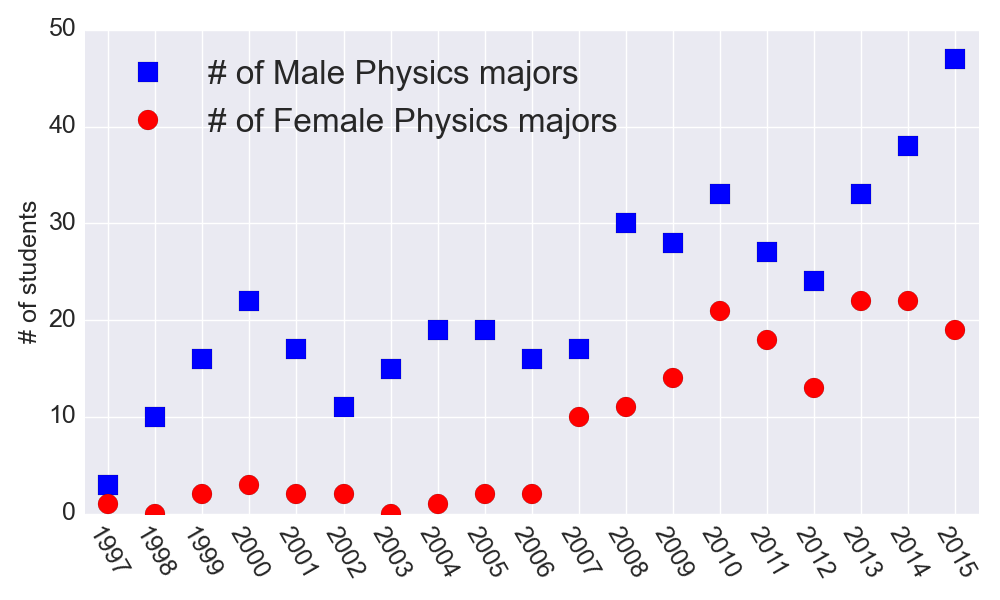
\includegraphics[height=0.29\textheight]{dept_plot.png}
\caption{The growth of the Physics department, particularly among women, has
  been striking over the last 10 years.  This is due in part to the high-level
  of engagement that the faculty have in involving students in research projects
  and in proactively recruiting and retaining young women scientists.
\label{fig:dept}}
\end{SCfigure}

\section{Department of Physics \& Astronomy}
			
The Department of Physics \& Astronomy aims to develop in its students a
comprehensive grasp of the principles of physics. The program emphasizes the
concepts and techniques that have led to our present state of understanding of
the physical universe. Placed in the context of a liberal arts environment, the
generality and applicability of the physics curriculum give physics majors three
broad options upon graduation. Students are well-prepared to pursue graduate
study in physics, astrophysics, or a related field; to embark immediately upon a
professional career in science; or to enter one of the numerous careers which
require or are enhanced by a broad knowledge of science in today's technological
society.
					
The department also offers a curriculum for students interested in teaching,
minors in astrophysics and computational science, and a 3/2 Engineering Program
through an articulation agreement with Clarkson University, Rensselaer
Polytechnic Institute (RPI), and Binghamton University.  The 3/2 program leads
to a B.S. in Physics and a B.E. in electrical, mechanical, civil, biomedical,
aeronautical, nuclear or materials engineering.  Programs leading to a Master’s
degree are also available through RPI and Union Graduate College.

%The Department offers a B.S. degree in Physics. We also offer a degree in
%Physics (Biological/Chemical Sciences Track), which allows students with
%interests in medicine or similar fields to complete a physics degree with
%somewhat different auxiliary courses. The Department has just ceased to offer a
%separate Physics Education major which had slightly reduced requirements, as
%this was not acceptable to New York State. Our majors can and do pursue
%certification to teach physics at the 7 − 12 grade level; this is now in
%addition to the full requirements of the physics major.

%Our mission is to develop in our students a comprehensive grasp of the
%principles of physics, emphasizing the concepts and techniques that have led to
%our present understanding of the state of the universe. In this manner, we
%provide students with a strong foundation in physics that is necessary for their
%pursuit of graduate education or careers in industry, research, education,
%engineering, health professions or other interdisciplinary fields. We strive to
%provide our faculty with career and research opportunities for their scholarly
%development and provide the college and community with a resource of knowledge
%and professional contribution.
				
Siena is a small liberal arts college that emphasizes teaching excellence, small
class sizes, and close student-faculty connections. Unlike many comparable
schools, Siena's Physics \& Astronomy Department also has a very strong research
program, with many federally funded projects. Dr. John Cummings, the current
Dean of Science, is funded by the NSF to work on neutrino physics at Daya Bay,
China (NSF PHY-0901954); Dr. Rose Finn is an NSF CAREER Fellow (Award 0847430);
Dr. Matt Bellis is funded by the NSF to search for new physics using data from
the LHC/CMS detector; and Dr. Graziano Vernizzi is funded to work on a variety
of computational biophysics problems through the Department of Defense.  In
addition, Drs. Larry Medsker, Rose Finn, and Allan Weatherwax share an NSF
S-STEM grant (DUE 0728452), and Dr. Medsker and Dr. Michele McColgan share an
NSF Robert Noyce Teacher Scholarship Program grant (DUE-1136322).  Finally,
Drs. Finn and Medsker recently completed a Clare Boothe Luce grant which
provided scholarships for women majoring in STEM areas.

Because of these and other efforts, the department has experienced an exciting
period of growth and revitalization, including five new faculty members in the
last seven years.  The result is a fairly young, active faculty who are leading
exciting research programs in astrophysics, biophysics, computational physics,
physics education research, biophysics, and atomic and particle physics. An
immediate benefit of the increase in the level of faculty research is a
corresponding increase in student engagement in these research endeavors.

The strength of our research program reflects a dramatic transformation of the
department over the past decade, accomplished through a focused emphasis on
excellence in STEM education supported by faculty research that integrates
undergraduates in ways that enable them to make meaningful contributions to the
field. These changes have enhanced our ability to recruit new students.  The
number of physics majors has increased dramatically during the last decade from
an average of 16 between 1997 and 2006 to 93 as of Fall 2015. The number of
female majors increased from an average of 1.5 to about 31 over that same time
period, constituting 33\% of our current group of majors (see Figure~1).

%Finally, the faculty strives to foster a sense of community within the
%Department, and we feel this has positively impacted our ability to recruit and
%retain students.

%The strength of our research program reflects a dramatic transformation of the
%department over the past decade, accomplished through a focused emphasis on
%excellence in STEM education supported by faculty research that integrates
%undergraduates in ways that enable them to make meaningful contributions to the
%field. These changes have enhanced our ability to recruit new students and the
%number of physics majors increased from an average of 16 between 1997 and 2006
%to 93 as of fall 2015. The number of female majors increased from an average of
%1.5 to about 31 over that same time period.

The transformation of Physics \& Astronomy at Siena College is a testament to
strategic vision, research-intensive faculty who love teaching, a focus on
undergraduate research, and the critical importance of NSF funding for basic
research and undergraduate STEM education.

%The administration at Siena College is fully supportive of faculty research
%efforts, willingly reducing the normal teaching load from 12 to 9 contact hours
%per semester for faculty actively pursuing research. The Physics department
%chair is proactive in creatively balancing the teaching load for faculty who are
%conducting grant-supported research.

\section{Impact of this proposal}

Successful funding of this proposal would have a significant impact on the PI's
ability to continue to offer cutting-edge research experiences to
undergraduates, and on the department and College's ability to recruit a
diversity of talented students.  Many of these opportunities would not normally
be available to a student at a small liberal arts college.

The interest in research opportunities among the students is significant, even
among freshmen and sophmores.  Every spring the faculty give presentations to
the students about current research opportunities, and there is always far more
demand than available resources, although many students are frequently willing
to gain experience through unpaid opportunities.

Students supported by this grant will move on to the next phase of their careers
more prepared for scientific and technological challenges.  Whether they pursue
astrophysics in graduate school or move on to technical careers, they will have
gained a wide range of practical skills which will serve them for life.
				
%The administration is supportive of an additional course reduction to 6 contact hours
%per semester if the faculty member can secure outside funding.

%As of 2008 to the present, the number of
%students participating in an undergraduate research experience
%more than tripled from 20 to 76 students (see Table.~\ref{tab:curca0}). 
%This represents a 74\%
%growth in undergraduate research participation by students over a
%five year period (see Table 1 for additional information). 

%\begin{table}[h]
    %\caption{Student Participation in Undergraduate Research Activities, 2008 - present.\label{tab:curca0}}
    %\begin{tabular}{c c c c c}
    %\hline
    %& {\bf Students on Sponsored} & {\bf Students on Sponsored} &   &  \\
     %& {\bf Funded Projects} & {\bf Funded Projects} & {\bf Siena College}  &   \\
    %{\bf Year} & {\bf (Academic Year)} & {\bf (Summer)} & {\bf Summer Scholars}  &  {\bf Total} \\
%\hline
%2007 &6 &5 &8 &20 \\
%2008 &9 &15&28&52 \\
%2009 &15&20&19&54 \\
%2010 &16&28&28&72 \\
%2011 &17&28&37&82 \\
%2012 &11&24&41&76 \\
%\end{tabular}
%\end{table}

%\begin{itemize}[itemsep=0pt,parsep=0pt,topsep=0pt,partopsep=0pt]
%    \item They will contribute to searches for new physics in some of the largest
%        and most complex scientific experiments on the planet.
%        Along the way, they will learn how nature works on a fundamental
%        level.
%    \item They will learn valuable skills such as computer programming (mostly
%        in Python), data analysis, and statistical techniques.
%    \item Siena students will travel to Cornell University, a top research university,
%        and interact with the graduate students and post-docs there.
%        This will motivate some of them to pursue graduate studies,
%        when previously they might not have.
%    \item Some select students will travel to Fermilab, the flagship national lab in the US for particle
%        physics. 
%    \item Some will also have the opportunity to travel overseas to CERN, the site
%        of the LHC and some of the most exciting scientific research in the world.
%    \item Students will learn about how large international scientific collaborations function.
%    \item Students will have the opportunity to be a co-author on a paper and present their
%        work at professional meetings.
%\end{itemize}

\end{document}
